% Santos. Supporting subsection for the Group Results.
\subsection{Dissipation and numerical resolution controls}\label{sec:additional-adiabatic-controls}
The archived \texttt{hyp\_z=4} cases at density gradients $0.6$ and $1.5$ retained approximately $54\%$ and $57\%$ of their initial perturbation free energy by $\widehat t=52$. With \texttt{hyp\_z=0}, both retained essentially their initial energy. Intermediate coefficients gave intermediate losses. The installed GENE build applies a parallel fourth-order hyperdiffusion stencil. The native energy writer places the parallel term in column 8 and total analytic $\mathrm dE/\mathrm d\widehat t$ in column 3. The integrated parallel term accounts for the measured loss to diagnostic precision. Potential amplitude still changes with nearly constant perturbation free energy. The field signal leaves a discrete damping rate and a unique real frequency unresolved.

\begin{center}\small
\begin{tabular}{@{}rrr@{}}
\toprule
\texttt{hyp\_z} & $E/E_0$ at $\omega_{n,D}=0.6$ & $E/E_0$ at $\omega_{n,D}=1.5$\\
\midrule
4 & 0.53881 & 0.57489\\
2 & 0.58137 & 0.62148\\
1 & 0.62351 & 0.66439\\
0 & 0.99997 & 0.99997\\
\bottomrule
\end{tabular}

\end{center}

\begin{figure}[H]\centering
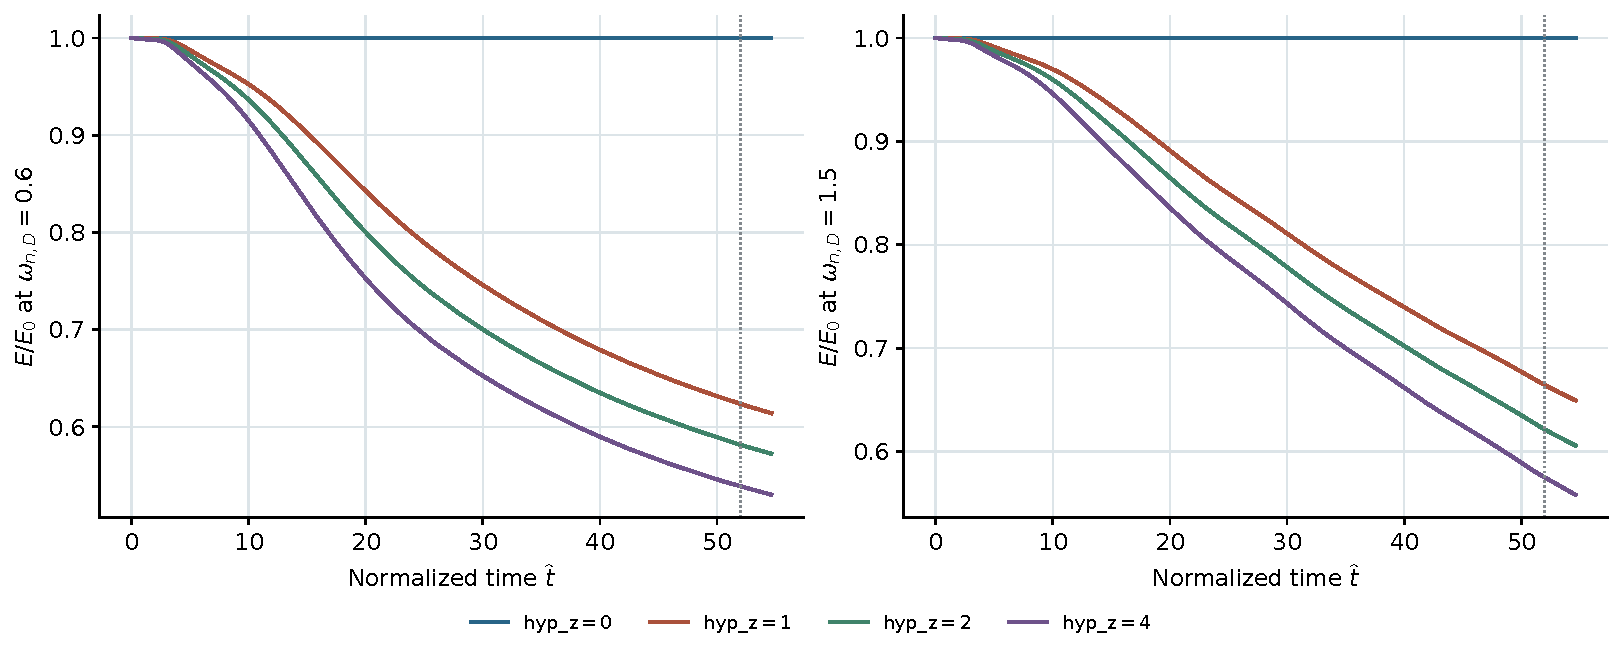
\includegraphics[width=\linewidth]{Figures/A_05_hyperdiffusion.pdf}
\caption{GENE free-energy sensitivity over matched times and timesteps. The vertical line marks the audit time $\widehat t=52$. Contributor: Santos.}
\label{fig:additional-hyperdiffusion}
\end{figure}

\begin{center}\small
\begin{tabular}{@{}rrrrrl@{}}
\toprule
Grid & $\Delta\widehat t$ & $\widehat t_{\rm rec,D}$ & Fit $\widehat\gamma$ & Fit $\widehat\omega_r$ & Assessment\\
\midrule
24/64/24 & 0.049657 & 56.55 & -0.0259 & -0.3371 & Unresolved\\
24/64/24 & 0.024829 & 56.55 & -0.0261 & -0.3372 & Unresolved\\
48/64/24 & 0.024829 & 56.55 & -0.0273 & -0.3339 & Unresolved\\
24/96/24 & 0.049657 & 85.27 & \textemdash & \textemdash & Rejected runaway\\
24/96/24 & 0.024829 & 85.27 & -0.0283 & -0.3346 & Unresolved\\
\bottomrule
\end{tabular}

\end{center}

At $\omega_{n,D}=1.5$, the $24/96/24$ run at the full timestep produced catastrophic energy growth with zero recorded drive. It was rejected despite GENE's native convergence flag. Spatial and velocity refinements are compared to a separate half-step $24/64/24$ control at nominal velocity extents. The finer velocity grid increases nominal recurrence time from about $56.55$ to $85.27$. The half-step $24/96/24$ run reached $\widehat t=75.01$ without a modal stop. The growth slope changes from $-0.0283$ over $44$--$52$ to $-0.0002$ over $64$--$74$, and the phase slope shifts from $-0.335$ to $-0.348$. Removing hyperdiffusion also exposes small short-wavelength ripples. At the common profile time near $52$, the fraction of potential spectral power in the upper quarter of the grid band is about $2.1\times10^{-3}$ on the $24$-point grid and $2.9\times10^{-5}$ on the $48$-point grid. Each fraction uses its grid's own Nyquist limit.
